\chapter{User Manual}

\section{Introduction}
This system was designed as a stock control system for a pub capable to deal with different type of stock and their different measurements. This system is designed to be used by regular bar staff with no programming experience, the user must have the basic knowledge of how to use a computer such as how to run a program, how to enter data into a program and how to close a program. the highest skill required will be knowing how to install an .exe file.

\section{Installation}
This system was designed to be run on a Windows 7 or Ubuntu 14.10 operating system

\subsection{Prerequisite Installation}
To be able to run this system you will have to install some other 3rd party software in order to get the system to run.

\subsubsection{Installing Python}
The first piece of software you will need is the latest version of python 3 this is easy to install but if you are not confidant in your ability here is a step by step guide.

\textbf{Step 1}

\begin{figure}[H]
    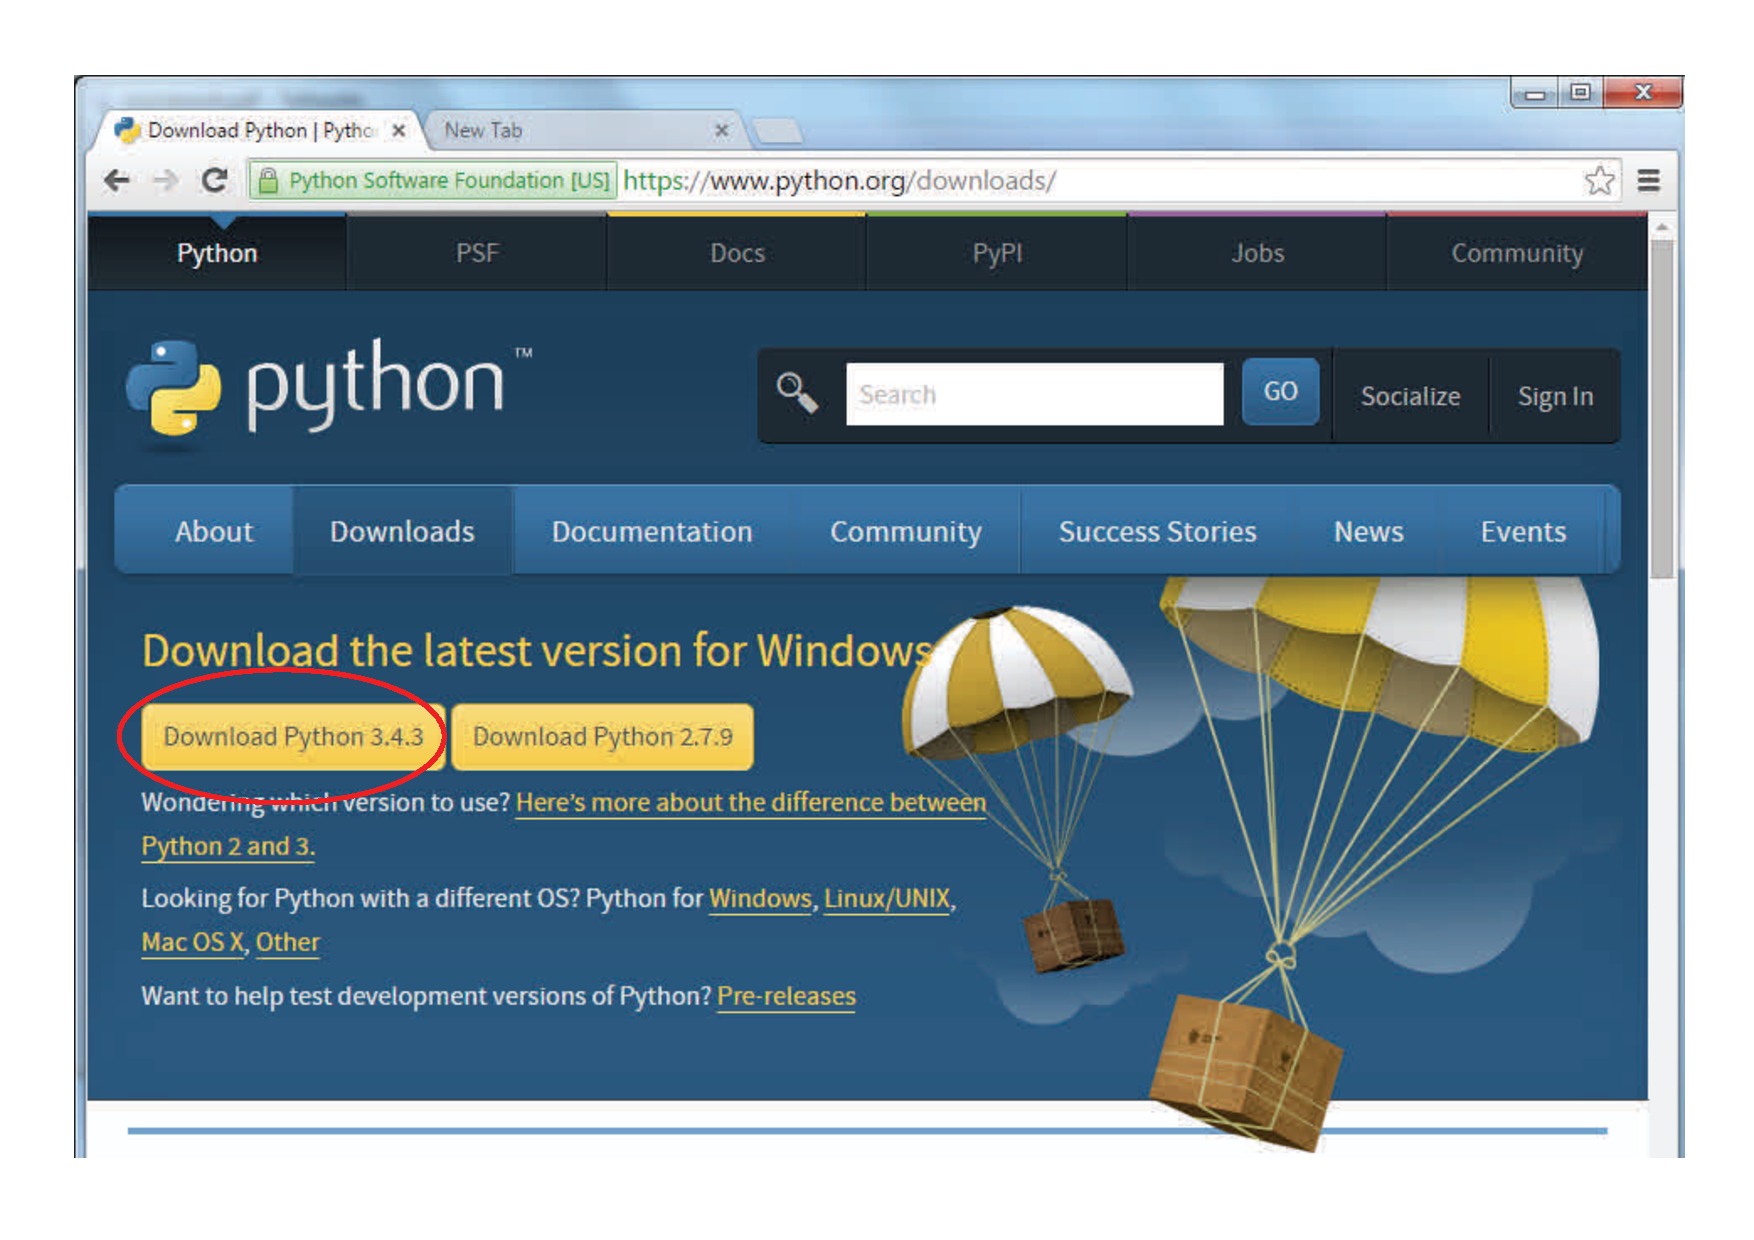
\includegraphics[width=\textwidth]{./Manual/images/python1.pdf}
    \caption{step 1 of installing python 3} \label{fig:installing python3 1}
\end{figure}

\textbf{Step 2}

\begin{figure}[H]
    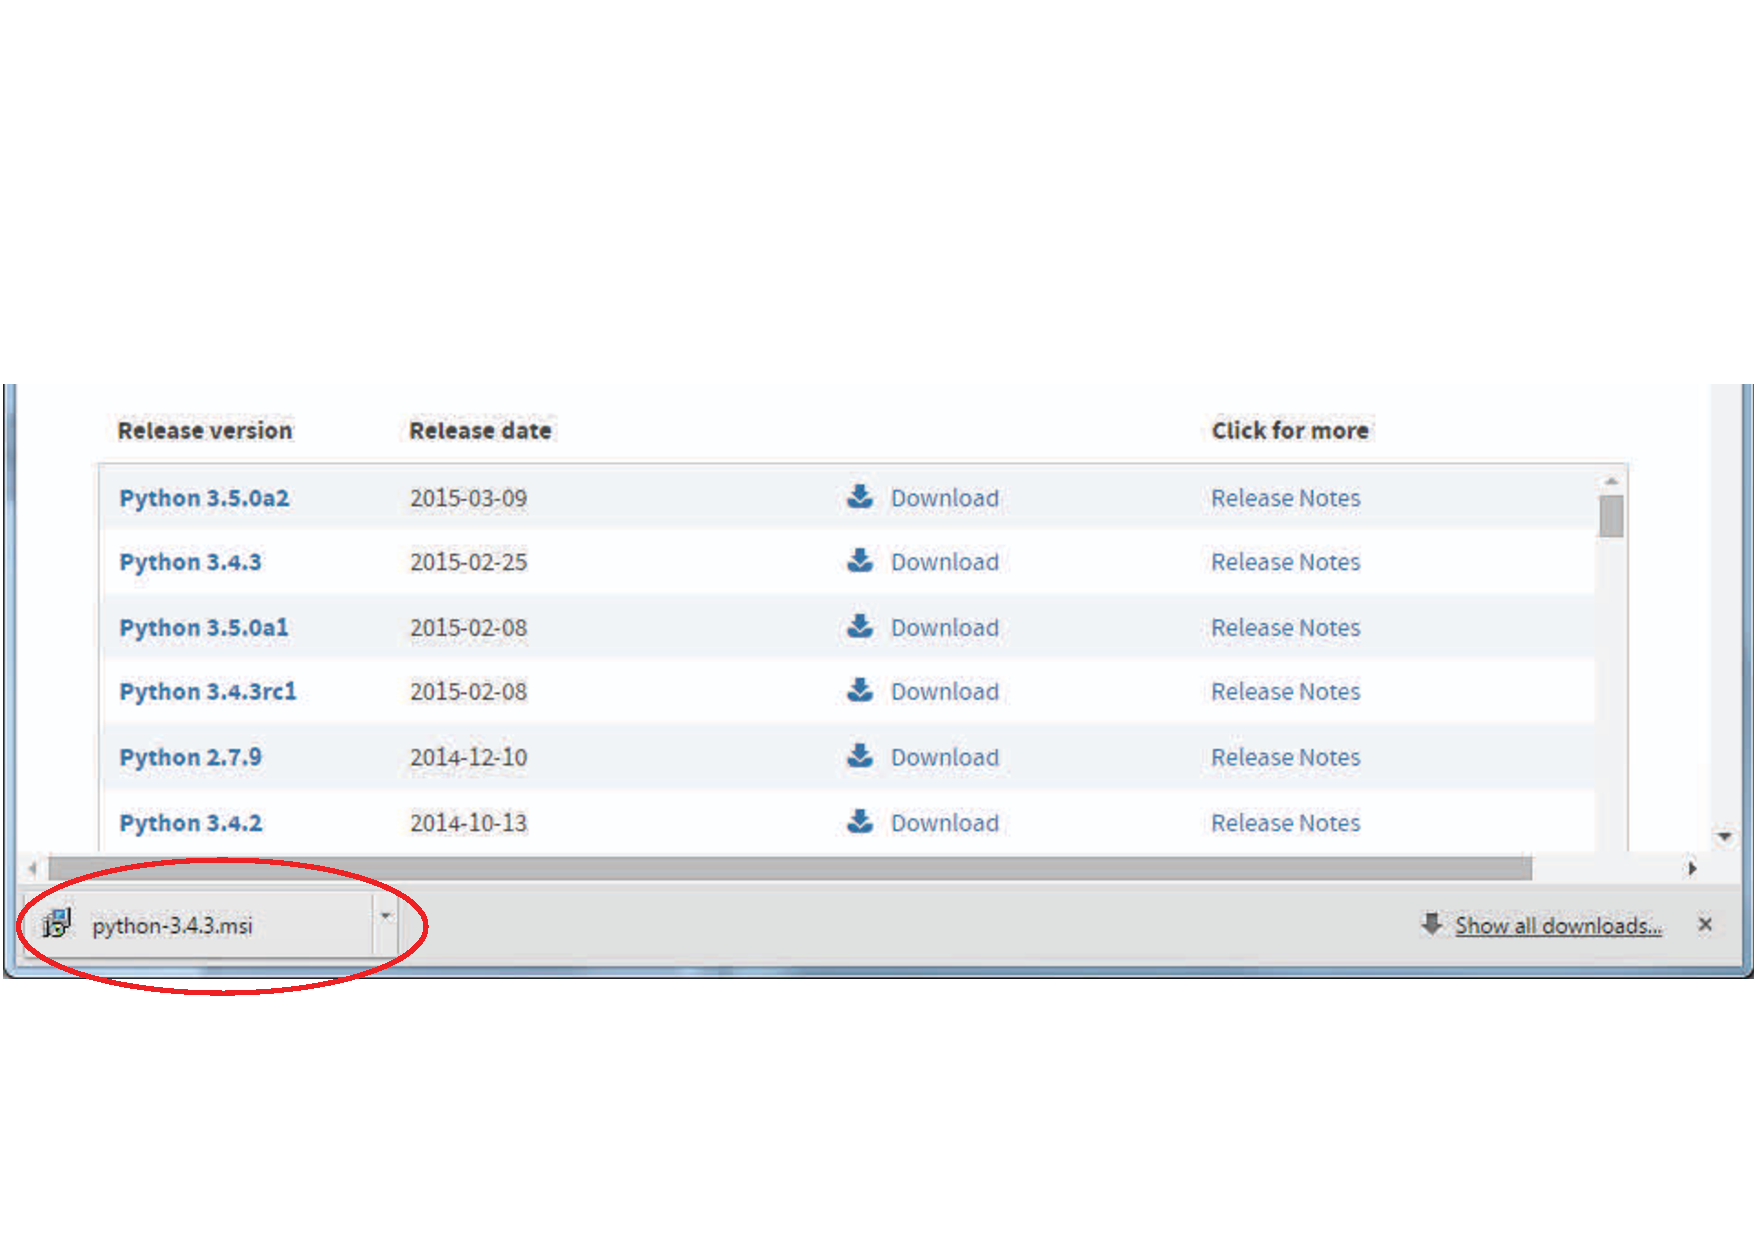
\includegraphics[width=\textwidth]{./Manual/images/python2.pdf}
    \caption{step 2 of installing python 3} \label{fig:installing python3 2}
\end{figure}

\textbf{Step 3}

\begin{figure}[H]
    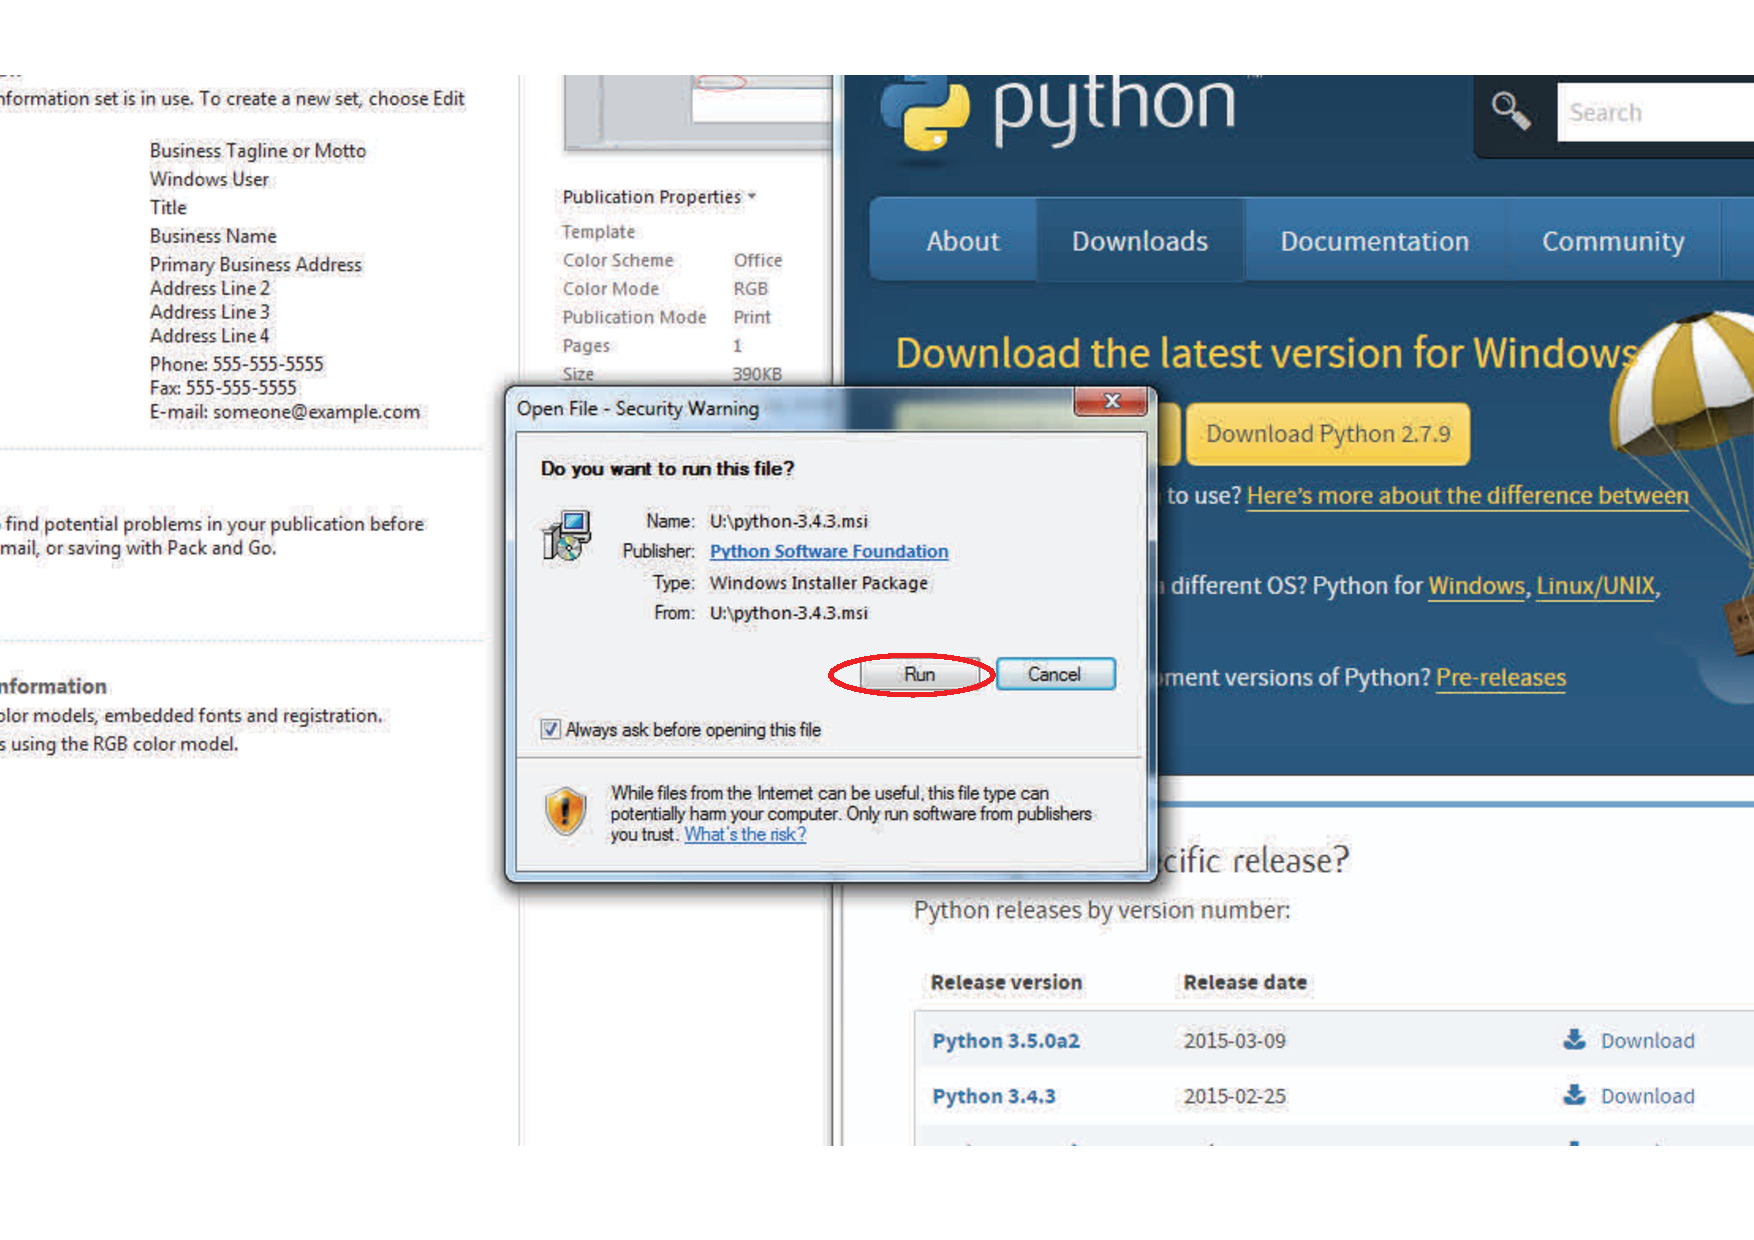
\includegraphics[width=\textwidth]{./Manual/images/python3.pdf}
    \caption{step 3 of installing python 3} \label{fig:installing python3 3}
\end{figure}

\textbf{Step 4}

\begin{figure}[H]
    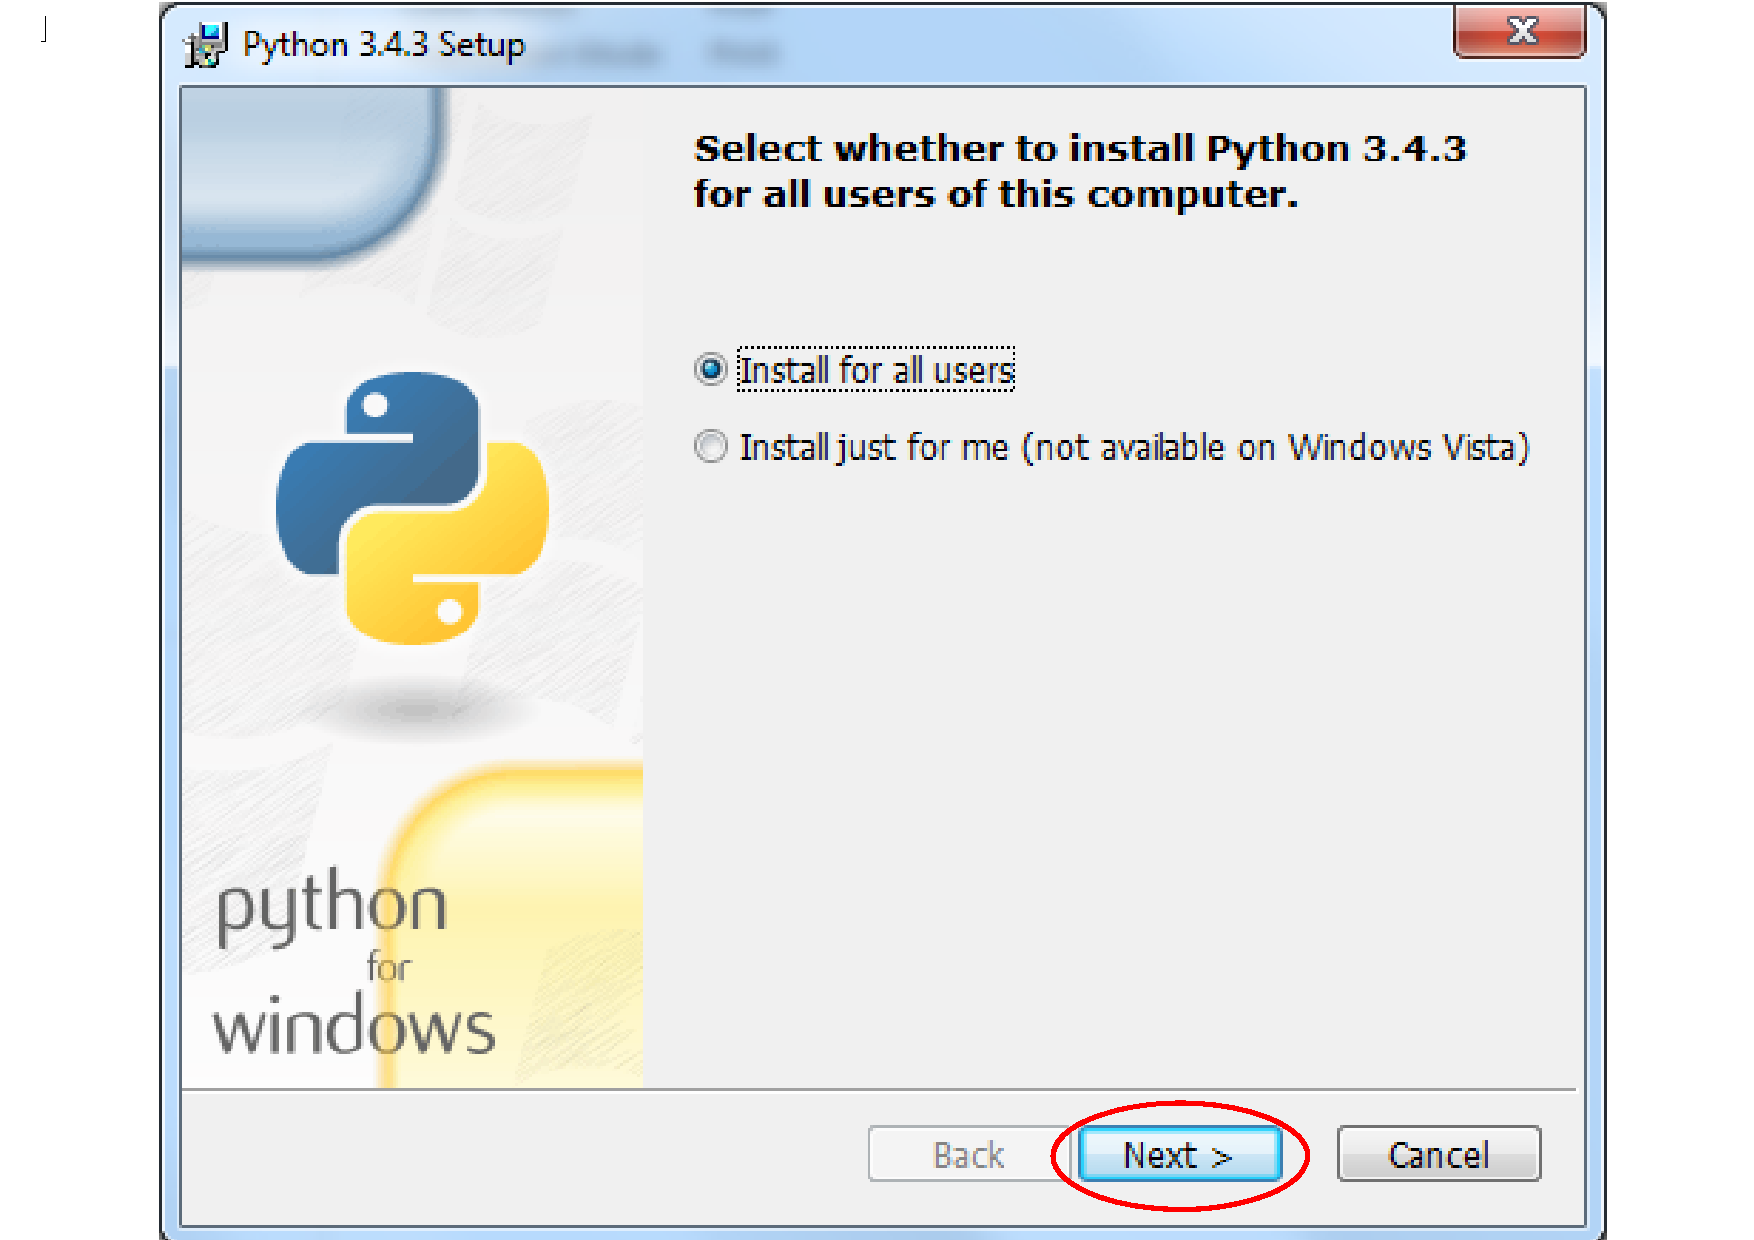
\includegraphics[width=\textwidth]{./Manual/images/python4.pdf}
    \caption{step 4 of installing python 3} \label{fig:installing python3 4}
\end{figure}

\textbf{Step 5}

\begin{figure}[H]
    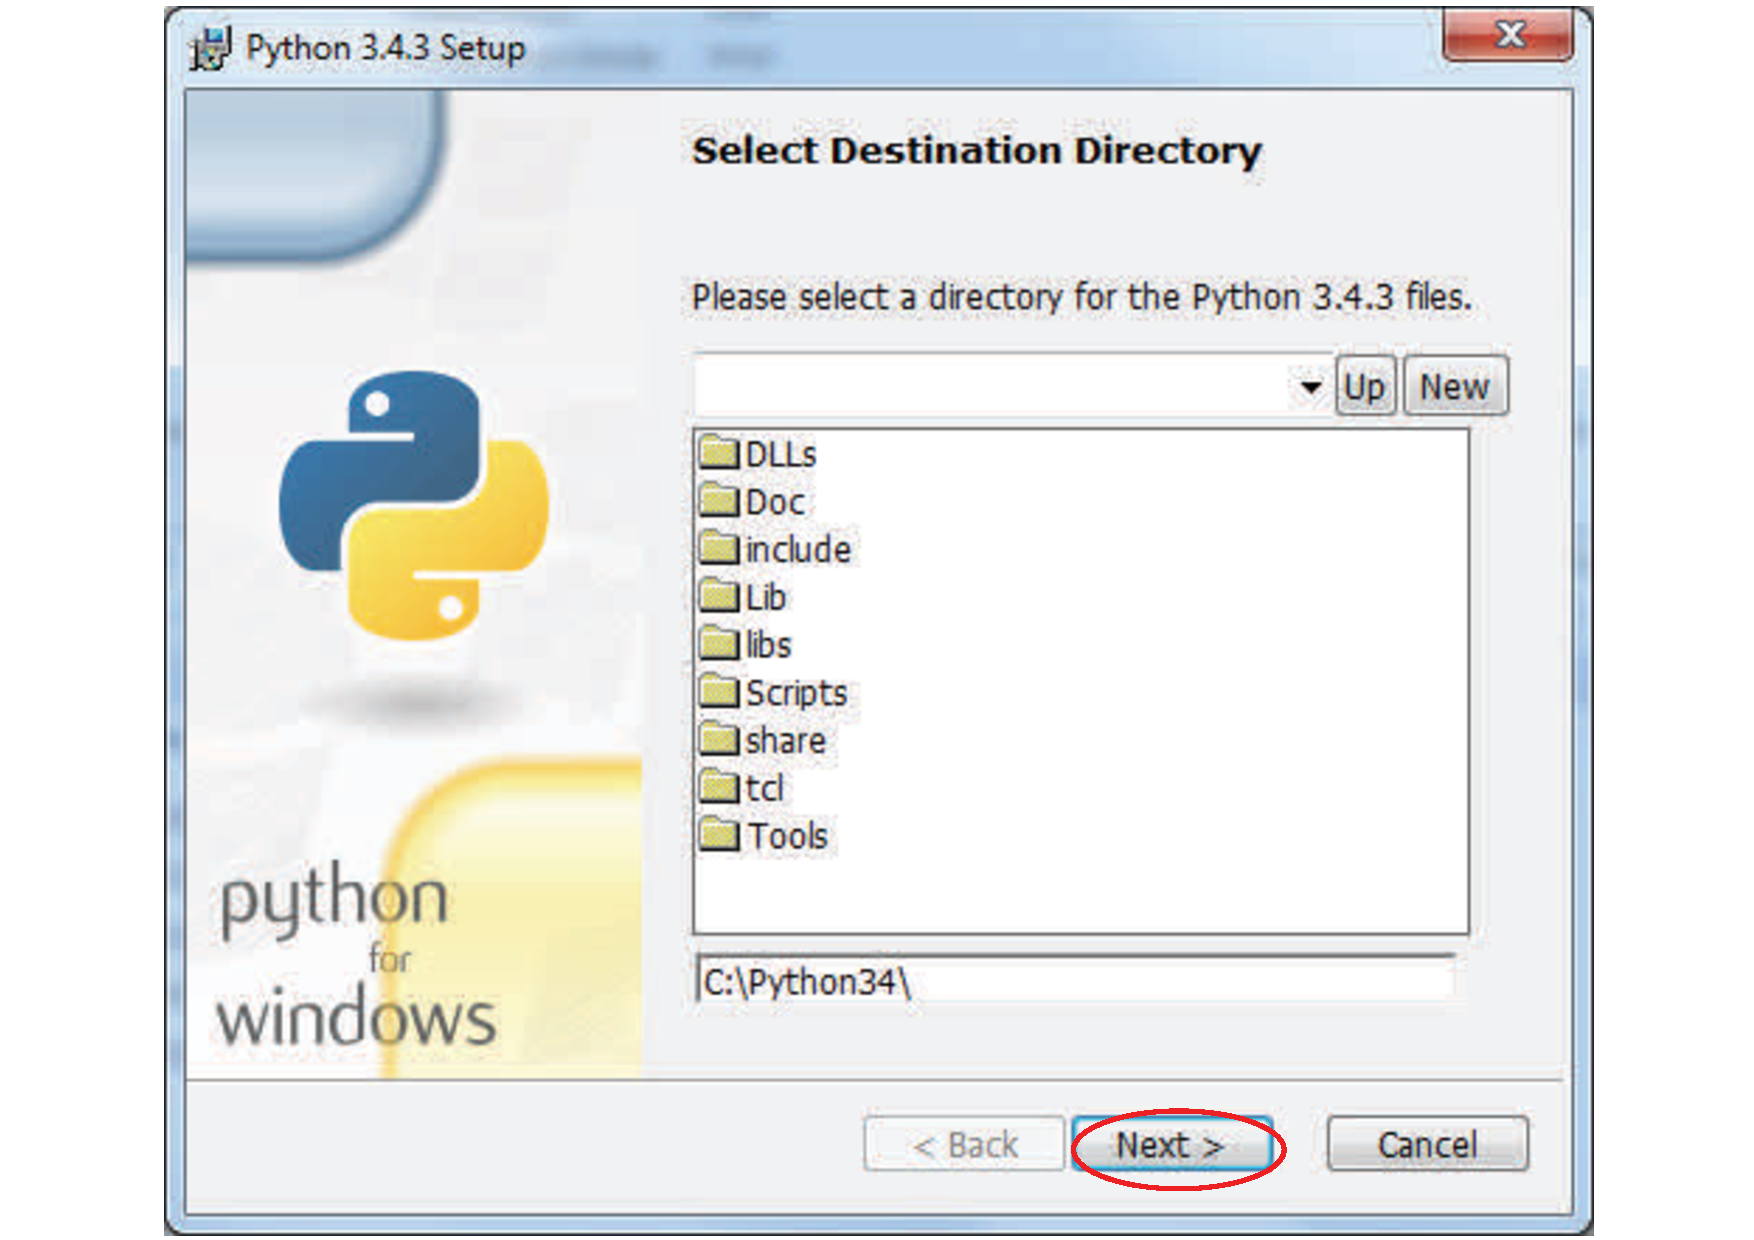
\includegraphics[width=\textwidth]{./Manual/images/python5.pdf}
    \caption{step 5 of installing python 3} \label{fig:installing python3 5}
\end{figure}

\textbf{Step 6}

\begin{figure}[H]
    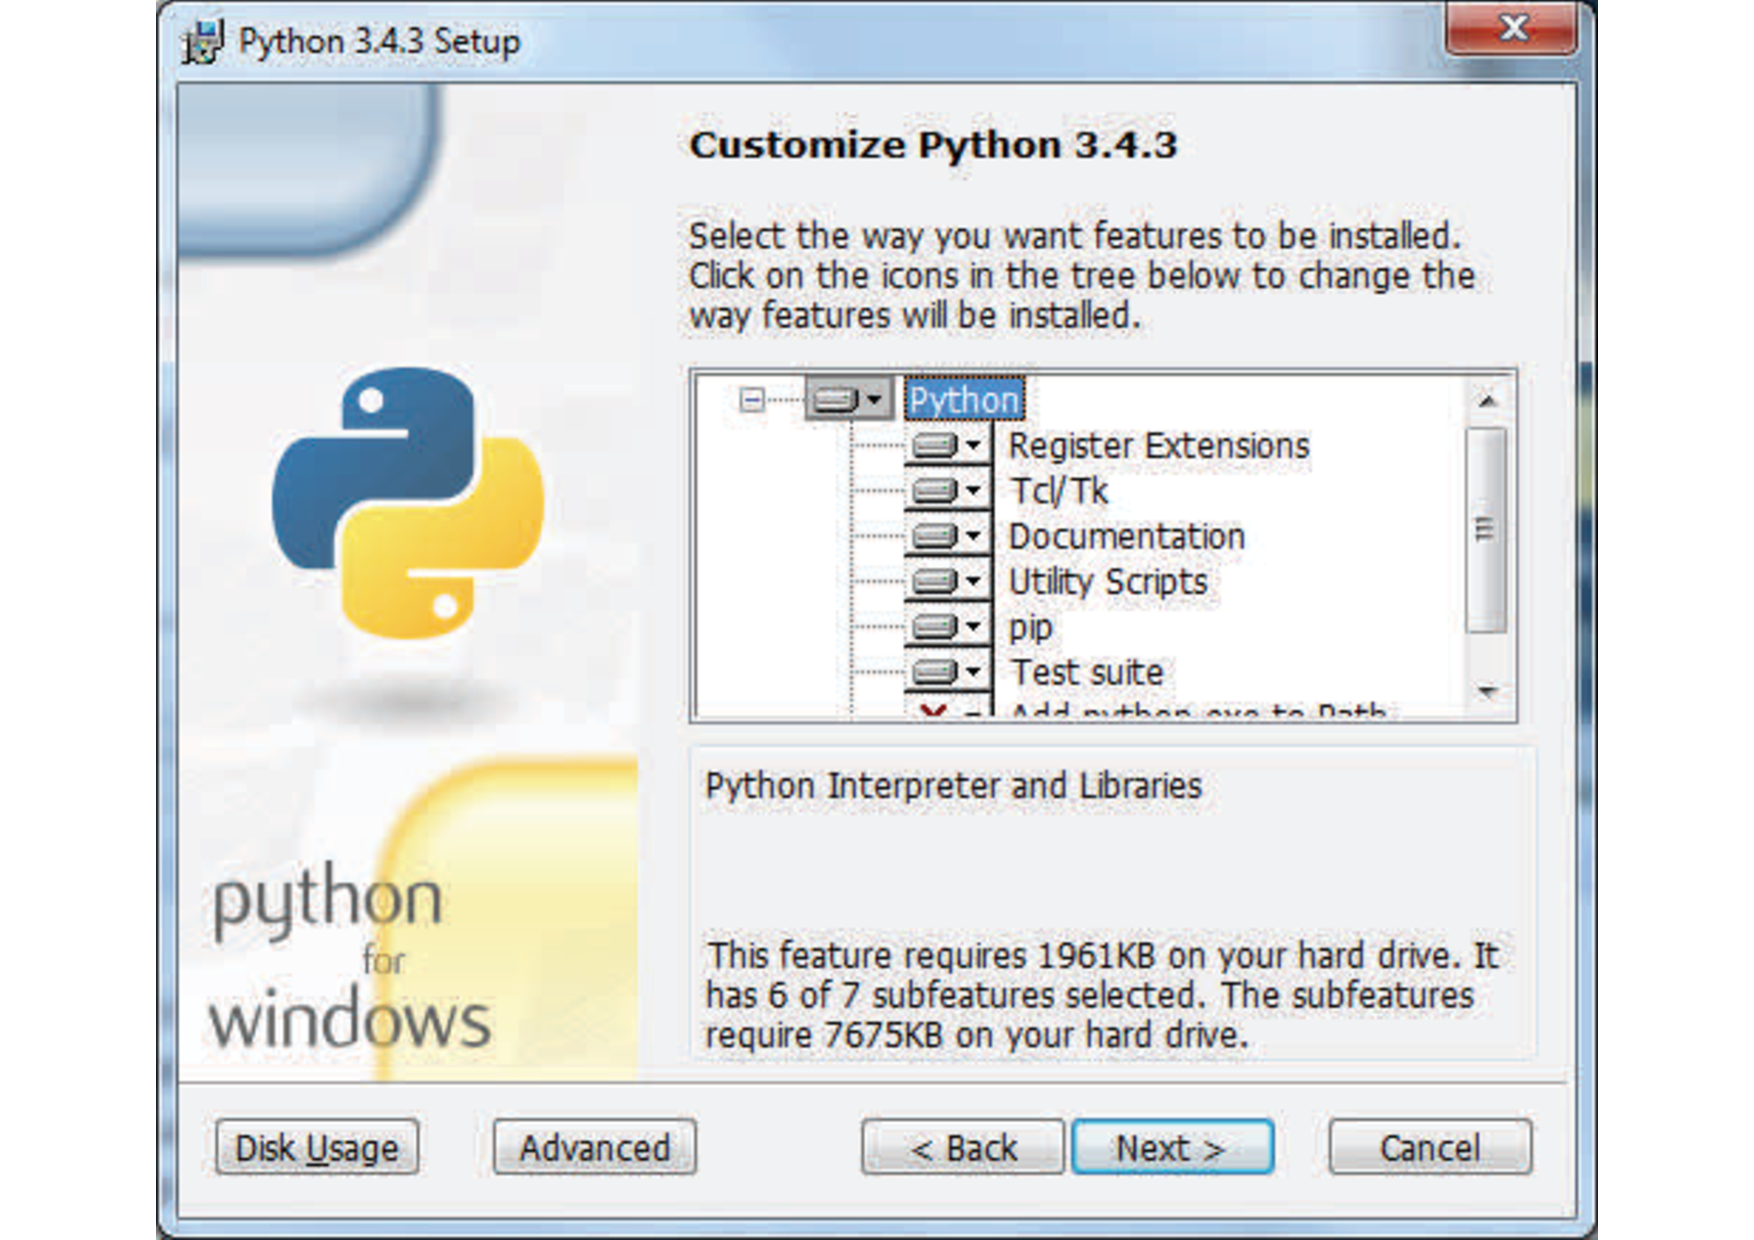
\includegraphics[width=\textwidth]{./Manual/images/python6.pdf}
    \caption{step 6 of installing python 3} \label{fig:installing python3 6}
\end{figure}

\textbf{Step 7}

\begin{figure}[H]
    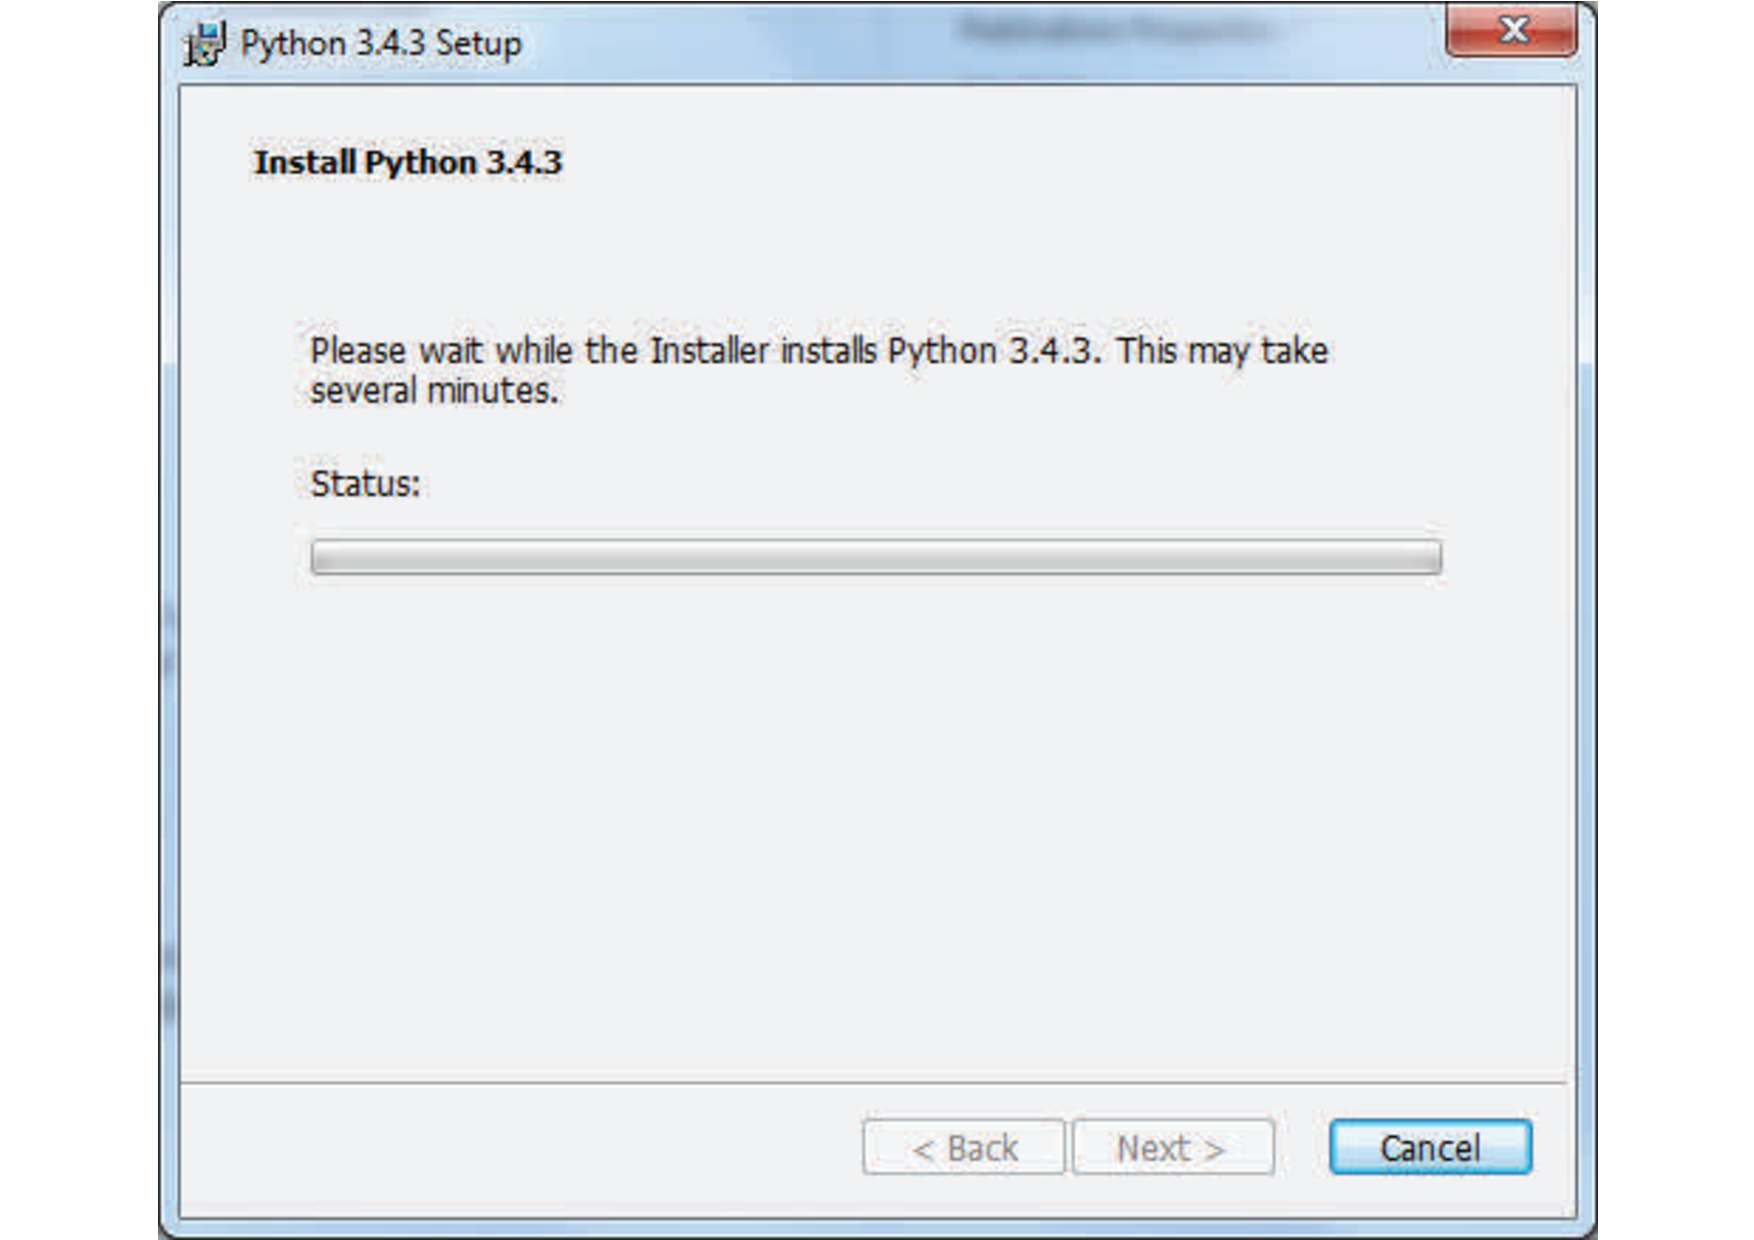
\includegraphics[width=\textwidth]{./Manual/images/python7.pdf}
    \caption{step 7 of installing python 3} \label{fig:installing python3 7}
\end{figure}

\textbf{Step 8}

\begin{figure}[H]
    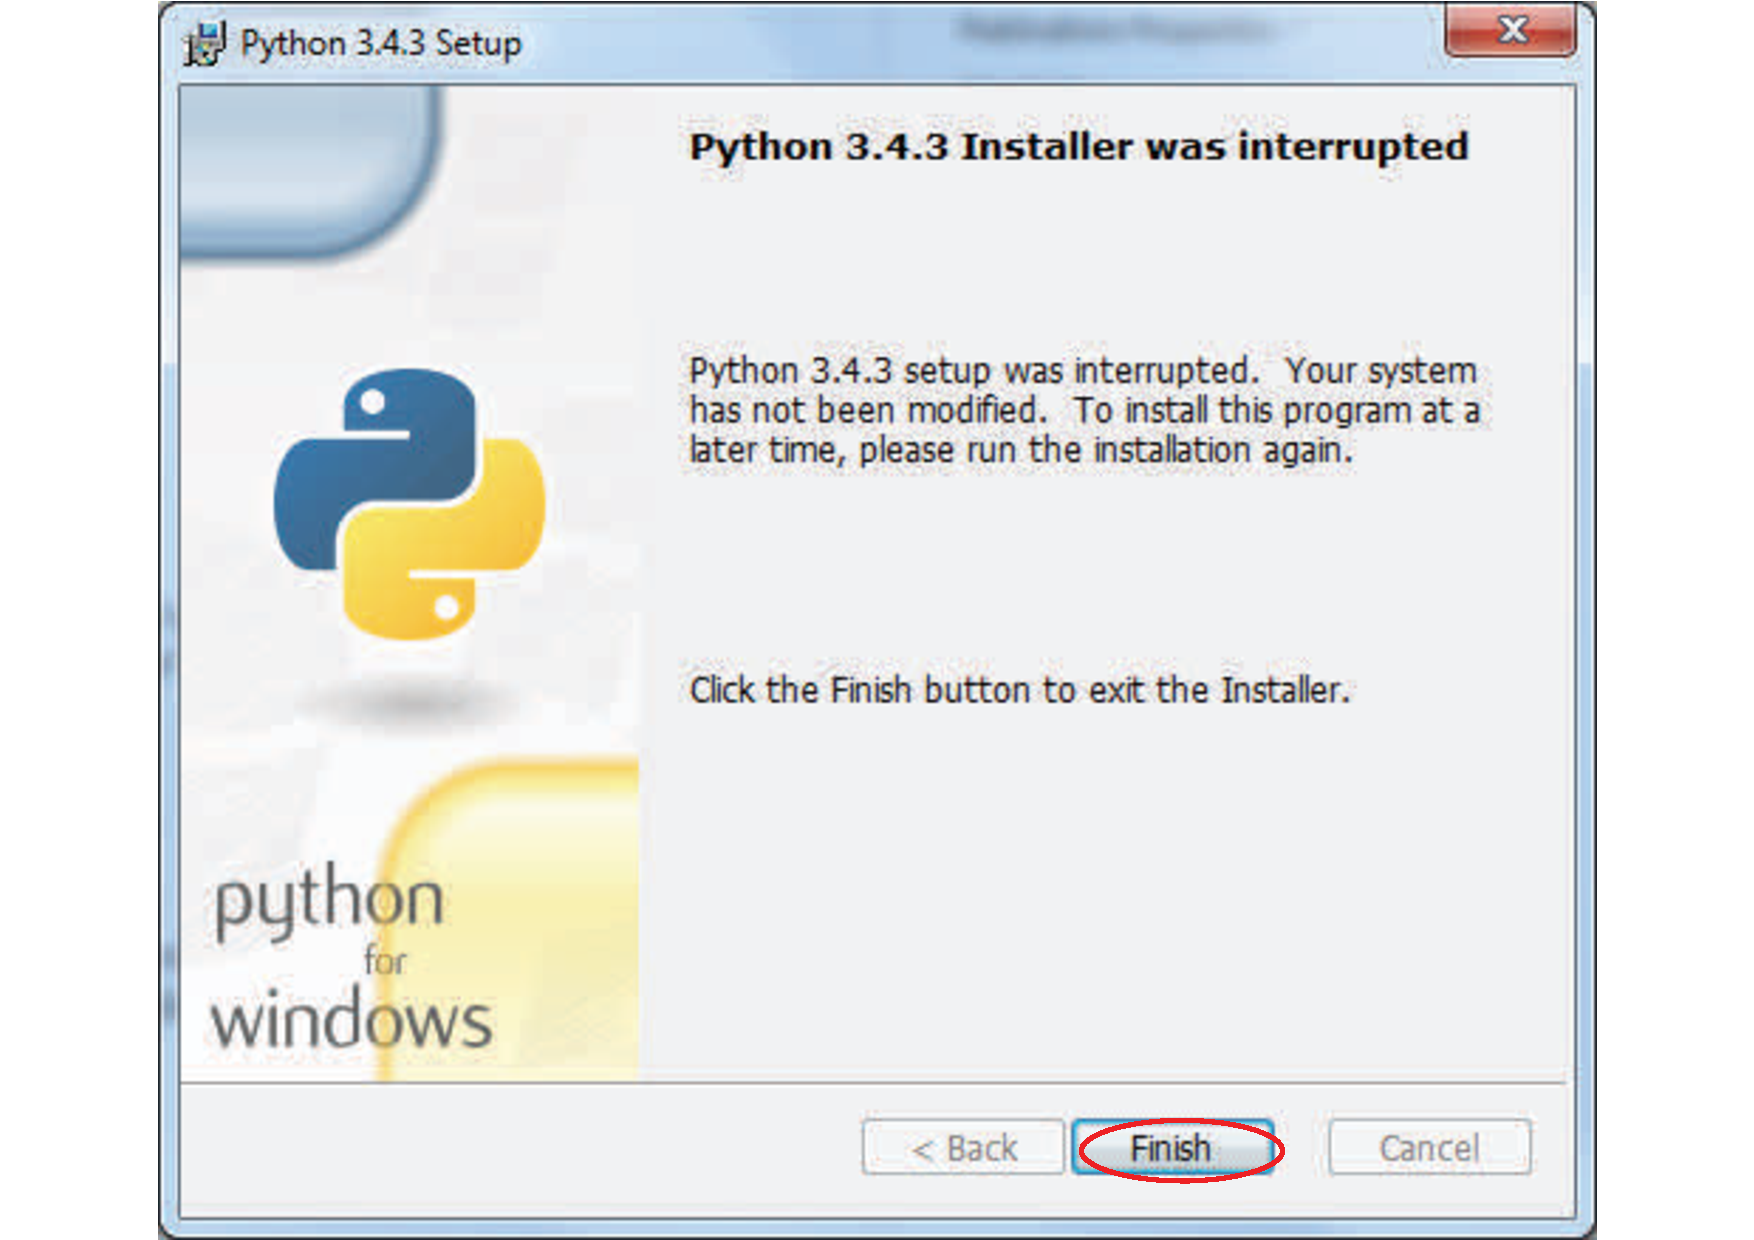
\includegraphics[width=\textwidth]{./Manual/images/python8.pdf}
    \caption{step 8 of installing python 3} \label{fig:installing python3 8}
\end{figure}

\subsubsection{Installing PyQt}

\subsubsection{Etc.}

\subsection{System Installation}

\subsection{Running the System}

\section{Tutorial}

\subsection{Introduction}

\subsection{Assumptions}

\subsection{Tutorial Questions}

%include as many subsubsections as necessary for each question in your list
\subsubsection{Question 1}

\subsubsection{Question 2}

\subsection{Saving}

\subsection{Limitations}

\section{Error Recovery}

%include as many subsections as necessary for each error
\subsection{Error 1}

\subsection{Error 2}

\section{System Recovery}

\subsection{Backing-up Data}

\subsection{Restoring Data}